% Options for packages loaded elsewhere
\PassOptionsToPackage{unicode}{hyperref}
\PassOptionsToPackage{hyphens}{url}
\PassOptionsToPackage{dvipsnames,svgnames,x11names}{xcolor}
\documentclass[
  12pt,
]{article}
\usepackage{xcolor}
\usepackage[margin=1in]{geometry}
\usepackage{amsmath,amssymb}
\setcounter{secnumdepth}{5}
\usepackage{iftex}
\ifPDFTeX
  \usepackage[T1]{fontenc}
  \usepackage[utf8]{inputenc}
  \usepackage{textcomp} % provide euro and other symbols
\else % if luatex or xetex
  \usepackage{unicode-math} % this also loads fontspec
  \defaultfontfeatures{Scale=MatchLowercase}
  \defaultfontfeatures[\rmfamily]{Ligatures=TeX,Scale=1}
\fi
\usepackage{lmodern}
\ifPDFTeX\else
  % xetex/luatex font selection
  \setmainfont[]{Times New Roman}
\fi
% Use upquote if available, for straight quotes in verbatim environments
\IfFileExists{upquote.sty}{\usepackage{upquote}}{}
\IfFileExists{microtype.sty}{% use microtype if available
  \usepackage[]{microtype}
  \UseMicrotypeSet[protrusion]{basicmath} % disable protrusion for tt fonts
}{}
\makeatletter
\@ifundefined{KOMAClassName}{% if non-KOMA class
  \IfFileExists{parskip.sty}{%
    \usepackage{parskip}
  }{% else
    \setlength{\parindent}{0pt}
    \setlength{\parskip}{6pt plus 2pt minus 1pt}}
}{% if KOMA class
  \KOMAoptions{parskip=half}}
\makeatother
\usepackage{graphicx}
\makeatletter
\newsavebox\pandoc@box
\newcommand*\pandocbounded[1]{% scales image to fit in text height/width
  \sbox\pandoc@box{#1}%
  \Gscale@div\@tempa{\textheight}{\dimexpr\ht\pandoc@box+\dp\pandoc@box\relax}%
  \Gscale@div\@tempb{\linewidth}{\wd\pandoc@box}%
  \ifdim\@tempb\p@<\@tempa\p@\let\@tempa\@tempb\fi% select the smaller of both
  \ifdim\@tempa\p@<\p@\scalebox{\@tempa}{\usebox\pandoc@box}%
  \else\usebox{\pandoc@box}%
  \fi%
}
% Set default figure placement to htbp
\def\fps@figure{htbp}
\makeatother
% definitions for citeproc citations
\NewDocumentCommand\citeproctext{}{}
\NewDocumentCommand\citeproc{mm}{%
  \begingroup\def\citeproctext{#2}\cite{#1}\endgroup}
\makeatletter
 % allow citations to break across lines
 \let\@cite@ofmt\@firstofone
 % avoid brackets around text for \cite:
 \def\@biblabel#1{}
 \def\@cite#1#2{{#1\if@tempswa , #2\fi}}
\makeatother
\newlength{\cslhangindent}
\setlength{\cslhangindent}{1.5em}
\newlength{\csllabelwidth}
\setlength{\csllabelwidth}{3em}
\newenvironment{CSLReferences}[2] % #1 hanging-indent, #2 entry-spacing
 {\begin{list}{}{%
  \setlength{\itemindent}{0pt}
  \setlength{\leftmargin}{0pt}
  \setlength{\parsep}{0pt}
  % turn on hanging indent if param 1 is 1
  \ifodd #1
   \setlength{\leftmargin}{\cslhangindent}
   \setlength{\itemindent}{-1\cslhangindent}
  \fi
  % set entry spacing
  \setlength{\itemsep}{#2\baselineskip}}}
 {\end{list}}
\usepackage{calc}
\newcommand{\CSLBlock}[1]{\hfill\break\parbox[t]{\linewidth}{\strut\ignorespaces#1\strut}}
\newcommand{\CSLLeftMargin}[1]{\parbox[t]{\csllabelwidth}{\strut#1\strut}}
\newcommand{\CSLRightInline}[1]{\parbox[t]{\linewidth - \csllabelwidth}{\strut#1\strut}}
\newcommand{\CSLIndent}[1]{\hspace{\cslhangindent}#1}
\setlength{\emergencystretch}{3em} % prevent overfull lines
\providecommand{\tightlist}{%
  \setlength{\itemsep}{0pt}\setlength{\parskip}{0pt}}
\usepackage[backend=biber,style=authoryear,maxcitenames=2,maxbibnames=99,doi=false,isbn=false,url=true]{biblatex}
\usepackage{caption}
\captionsetup[figure]{name=Fig.}
\addbibresource{References.bib}
\usepackage{float}
\usepackage{booktabs}
\floatplacement{figure}{H}
\usepackage{longtable}
\floatplacement{table}{H}
\renewcommand{\arraystretch}{1} % Default line spacing for tables
\usepackage{geometry}
\geometry{letterpaper, top=1in, bottom=1in, left=1in, right=1in}
\usepackage{setspace}
\singlespacing
\usepackage{indentfirst}
\setlength{\parindent}{2.5em}
\setlength{\parskip}{0.5em}
\fontsize{12}{15}\selectfont
\usepackage{graphicx}
\setkeys{Gin}{width=\linewidth}
\usepackage[utf8]{inputenc}
\usepackage[T1]{fontenc}
\usepackage{enumitem}
\DeclareUnicodeCharacter{2265}{\ensuremath{\geq}}
\DeclareUnicodeCharacter{2248}{\ensuremath{\approx}}
\newenvironment{eightpt}{\par\fontsize{8}{10}\selectfont}{\par}
\newenvironment{elevpt}{\par\fontsize{11}{10}\selectfont}{\par}
\usepackage{multicol}
\setlength{\columnsep}{12pt}      % space between columns
\setlength{\columnseprule}{0.1pt} % vertical rule between columns
\usepackage{caption}
\DeclareCaptionFont{eightpt}{\fontsize{8}{10}\selectfont}
\captionsetup[figure]{font=eightpt, labelfont={eightpt,bf},  labelsep=period}
\captionsetup[table]{font=eightpt, labelfont={eightpt,bf}, labelsep=period}
\usepackage[hidelinks]{hyperref}
\urlstyle{same}
\hypersetup{breaklinks=true}
\hypersetup{colorlinks=true, linkcolor=blue, citecolor=blue, urlcolor=blue}
\usepackage{pdflscape}
\usepackage{booktabs}
\usepackage{float}
\usepackage{longtable}
\usepackage{array}
\usepackage{multirow}
\usepackage{wrapfig}
\usepackage{colortbl}
\usepackage{pdflscape}
\usepackage{tabu}
\usepackage{threeparttable}
\usepackage{threeparttablex}
\usepackage[normalem]{ulem}
\usepackage{makecell}
\usepackage{xcolor}
\usepackage{bookmark}
\IfFileExists{xurl.sty}{\usepackage{xurl}}{} % add URL line breaks if available
\urlstyle{same}
\hypersetup{
  colorlinks=true,
  linkcolor={Maroon},
  filecolor={Maroon},
  citecolor={Blue},
  urlcolor={blue},
  pdfcreator={LaTeX via pandoc}}

\author{}
\date{\vspace{-2.5em}}

\begin{document}

\begin{center}
\textbf{Semi-Supervised and Supervised Machine Learning Approaches to Predicting Fluvial Mesohabitats from Satellite Data}

\noindent
Elvin Cordero$^{1,2}$ and Aubrey Harris$^3$
\end{center}

\noindent \textbf{Affiliation:}

\noindent $^1$ Department of Marine Sciences, University of Puerto
Rico-\textnormal{Mayag\"uez}, PO Box 9000 \textnormal{Mayag\"uez}, PR 00681, USA

\noindent $^2$ SeaMount Geospatial Labs, Brooklyn, NY, USA

\noindent $^3$ US Army Corps of Engineers, Engineering Research and Development Center, Environmental Laboratory, Albuquerque, NM, USA

\noindent \textbf{Corresponding Author:} Aubrey Harris
\begin{itemize}[leftmargin=*]
    \item \href{mailto:Aubrey.E.Harris@USACE.army.mil}{Aubrey.E.Harris@USACE.army.mil}
    \item Phone: +1 (505) 342-3329
\end{itemize}

\noindent \textbf{Research Domain:} Remote Sensing, Machine Learning, Ecosystem Modeling

\noindent \textbf{Funding Information:} US Army Corps of Engineers’ Aquatic and Nuisance Species Research Program focus on Next Generation Ecological Modeling. This research was supported in part by an appointment to the Department of Defense (DOD) Research Participation Program administered by the Oak Ridge Institute for Science and Education (ORISE) through an interagency agreement between the U.S. Department of Energy (DOE) and the DOD. ORISE is managed by Oak Ridge Associated Universities (ORAU) under DOE contract number DE-SC0014664.

\noindent \textbf{Highlights:}
\begin{itemize}[leftmargin=*]
    \item Semi-supervised K-means achieved 88\% accuracy in mesohabitat classification.
    \item Demonstrates an effective, accessible change detection workflow for assessing mesohabitat change from sediment mobilization using Open-Source tools.
    \item Combined supervised and unsupervised methods improves classification flexibility.
\end{itemize}

\noindent \textbf{Date:} November 23, 2025

\newpage

\section*{Abstract}\label{abstract}
\addcontentsline{toc}{section}{Abstract}

High-cadence satellite data creates new opportunities for riverscape
assessment provided that analyses are fast, reproducible, and robust to
changing flow. This study evaluates open-source workflows for
mesohabitat mapping from optical imagery, contrasting a semi-supervised
clustering approach with a class-weighted supervised random forest. Two
complementary targets were considered: (i) inundation (water
vs.~non-water) within the river corridor and (ii) direct prediction of
hydraulically derived mesohabitat labels. Using PlanetScope
(\textasciitilde3 m) and Landsat-9 (30 m) imagery co-registered to
HEC-RAS outputs, the semi-supervised pipeline recovered inundation with
high agreement (accuracy = 0.88; kappa = 0.73) and was less sensitive to
sensor resolution than the supervised baseline. Time-series analysis
revealed a moderate negative association between surface water and bare
land area, consistent with flow-driven exposure and sediment
mobilization. In a leave-one-date-out evaluation across seven flow
conditions, direct mesohabitat classification from PlanetScope features
achieved modest cross-date performance (mean per-pixel accuracy ≈
0.20--0.22; mean kappa ≈ 0.02--0.03) but produced spatially coherent
patterns (e.g., pools along thalweg, high-velocity units at
constrictions), indicating learnable signal from image features alone.
Results demonstrate that open, lightweight pipelines can deliver
decision-ready inundation products today and provide a proof-of-concept
for image-based mesohabitat mapping. Pathways to higher accuracy include
restoring native spatial resolution (\textasciitilde3 m), incorporating
texture and morphological context, and fusing hydraulic predictors,
enabling routine, basin-scale monitoring of mesohabitat dynamics.

\noindent \textbf{Keywords:} Machine Learning, Google Earth Engine,
Mesohabitats, Land Classification, Remote Sensing

\pagenumbering{gobble}

\section{Introduction}\label{introduction}

High-resolution remote sensing (RS) has transformed observation of
riverscapes by enabling routine, synoptic mapping of water extent,
channel morphology, and habitat structure at organism-relevant spatial
grains and operational cadences (Marcus and Fonstad, 2010). Expanding
public and commercial image archives, cloud platforms, and open
analytical ecosystems now support ecological assessment at spatial and
temporal resolutions that field data collection campaigns alone cannot
sustain (Cavender-Bares et al., 2022). Field surveys remain
indispensable yet are constrained by access, safety, and personnel,
particularly during high flows or across difficult floodplain terrain,
creating persistent gaps in coverage and frequency (Calderon and An,
2016; Griffin and Lasko, 2020; Johansen et al., 2022; Suir et al.,
2023).

Within hierarchical river habitat frameworks, mesohabitats (e.g., pools,
riffles/glides, runs/raceways) occupy the intermediate scale between
microhabitats and reaches and exert first-order control on hydraulics,
sediment processes, and aquatic assemblages (Aadland, 1993; Wegscheider
et al., 2020). The spatial configuration of these mesohabitats shifts
with discharge and sediment dynamics, highlighting the need for mapping
approaches that are both spatially extensive and temporally responsive
(Van Rooijen and Lotsari, 2024; Zaimes et al., 2021). Conventional
delineation via expert field mapping and ecohydraulic modeling can
achieve high fidelity but is typically limited to short river segments
and sparse flow snapshots given the demands for detailed topography,
boundary conditions, and calibration (Harris et al., 2024; Schwartz,
2016; Wiest et al., 2024).

Remote sensing provides an opportunity to upscale mesohabitat assessment
by exploiting spectral, textural, and morphological signals. Habitat
studies are increasingly using RS tools such as supervised/unsupervised
land-cover classification, spectral indices (e.g., Normalized Difference
Vegetation Index {[}NDVI{]}, Normalized Difference Water Index
{[}NDWI{]}, Normalized Burn Ratio {[}NBR{]}), texture metrics, and
Digital Elevation Model (DEM) derived context (e.g.~slope, curvature)
(Demir et al., 2018; Farwell et al., 2021; Ganesh et al., 2023; Jin et
al., 2021; Li et al., 2018; McKay et al., 2022; Niedballa et al., 2022;
Suttidate et al., 2023). Change-detection frameworks further enable
assessment of temporal dynamics across seasons and events (Choukiker and
Dohare, 2021; Lim et al., 2018; Romero et al., 2016; Zimmermann et al.,
2007).

A large body of work has leveraged Geographic Object-Based Image
Analysis (OBIA) to map riverscape units by coupling image segmentation,
spectral features, and contextual/topographic constraints. Hierarchical,
multiscale OBIA that fuses very high resolution (VHR) imagery with LiDAR
has produced accurate maps of channels, bars, riparian vegetation, and,
in some cases, in-channel mesohabitats (Demarchi et al., 2016a, 2016b;
Kutz et al., 2022; Shabat and Tapamo, 2017). Yet performance can be
sensitive to segmentation parameters and scene complexity, with
transferability across dates, sites, and flow states often requiring
retuning, especially where specular reflection, turbidity, shadows, and
narrow channels degrade separability (Wang et al., 2019; Wurm et al.,
2019; Zhang et al., 2023).

Machine learning (ML) and deep learning have expanded capabilities by
learning features directly from data. Convolutional neural networks
(CNNs), classification and representation learning models; and other
classical ML models provide robust baselines and ensembles for
tabular/image features (Aggarwal, 2018; Howard and Gugger, 2020; Kuhn,
2008; Lantz, 2023; Ma et al., 2019; Thompson and Brodrick, 2021). In
fluvial contexts, deep learning networks at sub-meter resolution can
exploit texture and spatial context to classify water and hydraulically
relevant surface states---even with limited spectral bands---while
hybrid workflows integrating image-derived flow texture with terrain
cues have distinguished glides, riffles, and pools across discharge
conditions (Brostow et al., 2009; Moortgat et al., 2022; Romero et al.,
2016; Shashikant, 2019; Verma et al., 2021). These developments suggest
that mesohabitat categories may be predictable directly from imagery,
provided appropriate annotations and cross-date validation.

Sensor choice is important; coarser sensors (10--30 m) incur mixed
pixels in narrow channel widths, whereas most VHR constellations trade
spatial grain against temporal cadence. PlanetScope (\textasciitilde3 m,
near-daily) offers a pragmatic balance for riverscape monitoring and has
seen wide uptake across aquatic and terrestrial applications (Planet
Labs PBC, 2024). National aerial programs (e.g., National Agriculture
Imagery Program {[}NAIP{]}; U.S. Geological Survey {[}USGS{]} 1-m
orthoimagery) provide sub-meter data but at lower or irregular temporal
frequency, complicating multi-date analyses tied to flow (USDA, n.d.;
USGS, 2023a, 2023b, 2011). Persistent challenges include assembling
labeled datasets at scale, coping with class imbalance among
mesohabitats, and ensuring robustness to domain shifts in color,
turbidity, substrate, and illumination (Mandlik and Mundhe, 2018; Maskey
et al., 2018; Vahidi et al., 2023).

Despite substantial advances, an operational gap remains: can
mesohabitat types be predicted directly from satellite features across
streamflow regimes, without reliance on site-specific LiDAR or dense
field annotation, and with validation that is explicitly out-of-time and
hydrologically aware? Object-based pipelines often require site/timestep
retuning and can degrade under heterogeneous riverscape conditions
(i.e.~specular reflection, shadows, turbidity), limiting transferability
(Demarchi et al., 2016a, 2016b; Kutz et al., 2022; Zhang et al., 2023).
Deep learning and modern ML offer stronger representation capacity but
remain sensitive to label scarcity, class imbalance, and domain shift
across color/turbidity/illumination (Aggarwal, 2018; Fix and Hodges,
1989; Ma et al., 2019; Maskey et al., 2018; Vahidi et al., 2023; Wang et
al., 2019; Wurm et al., 2019). Moreover, ecohydraulic mapping at scale
is constrained by the cost and data demands of LiDAR-driven or fully
calibrated hydraulic models (Lindenschmidt and Carr, 2018; Schwartz,
2016). Because mesohabitat composition shifts with discharge, models
must respect flow dependence and test temporal generalization (Aadland,
1993; Harris et al., 2024). These considerations motivate a
label-efficient, imagery-first strategy that exploits high-cadence VHR
sources (e.g., Planet) for multi-date coverage while limiting
mixed-pixel issues typical of coarser sensors in narrow channel widths
(Planet Labs PBC, 2024; USGS, 2023c)

This study advances riverscape mapping by testing whether mesohabitat
classes can be inferred directly from high-resolution satellite features
across varying discharges, rather than relying on inundation proxies.
Focusing on the Big Blue--Kansas Rivers confluence (Manhattan, KS), the
work (i) establishes reach-scale baseline landcover land-use (LULC) and
mesoscale change products for context and continuity, and (ii) evaluates
image-based prediction of eight hydraulically defined mesohabitats using
PlanetScope imagery (Planet Labs PBC, 2024) due to its consistent,
near-same-day coverage of all modelled dates. The central objective is
to quantify how well satellite-only predictors recover mesohabitat
labels under temporally out-of-sample conditions and to benchmark those
results against the simpler inundation classification, delivering
categorical prediction maps and cross-date performance summaries
suitable for monitoring and management. All analyses are implemented
with open, reusable tooling to maximize transparency and
transferability.

\newpage

\section{Methodology}\label{methodology}

\subsection{Software \& Data
Requirements}\label{software-data-requirements}

The geospatial processing procedure was completed for the data prior to
the statistical analysis utilizing the R statistical language (R Core
Team, 2023). A suite of R spatial tools including the \emph{terra}, in
concert with the \emph{tidyterra} and \emph{rgee}, were used for the
data acquisition steps (Aybar et al., 2020; Hernangómez, 2023; Hijmans,
2024). The \emph{rgee} package is a nested wrapper that connects R to
the Google Earth Engine (GEE) Web REST API via the GEE Python API (Aybar
et al., 2024; Eltayeb Elmahal and Mahmoud Ibrahim Musa, 2023). The USGS
discharge data from the nearest sites on the Kansas River (\#6879100
Fort Riley and \#6887500 Wamego) and the Big Blue River (\#6887000
Manhattan) were downloaded by using the R package \emph{dataRetrievel}
(De Cicco et al., 2023) (Fig. \ref{fig:studyArea}b-c). The R package
\emph{tidymodels} was used to employ the ML methods (Kuhn and Wickham,
2020). Polygon drafting and editing was done in the QGIS geographic
information system software (QGIS Development Team, 2024).

\begin{figure}

{\centering 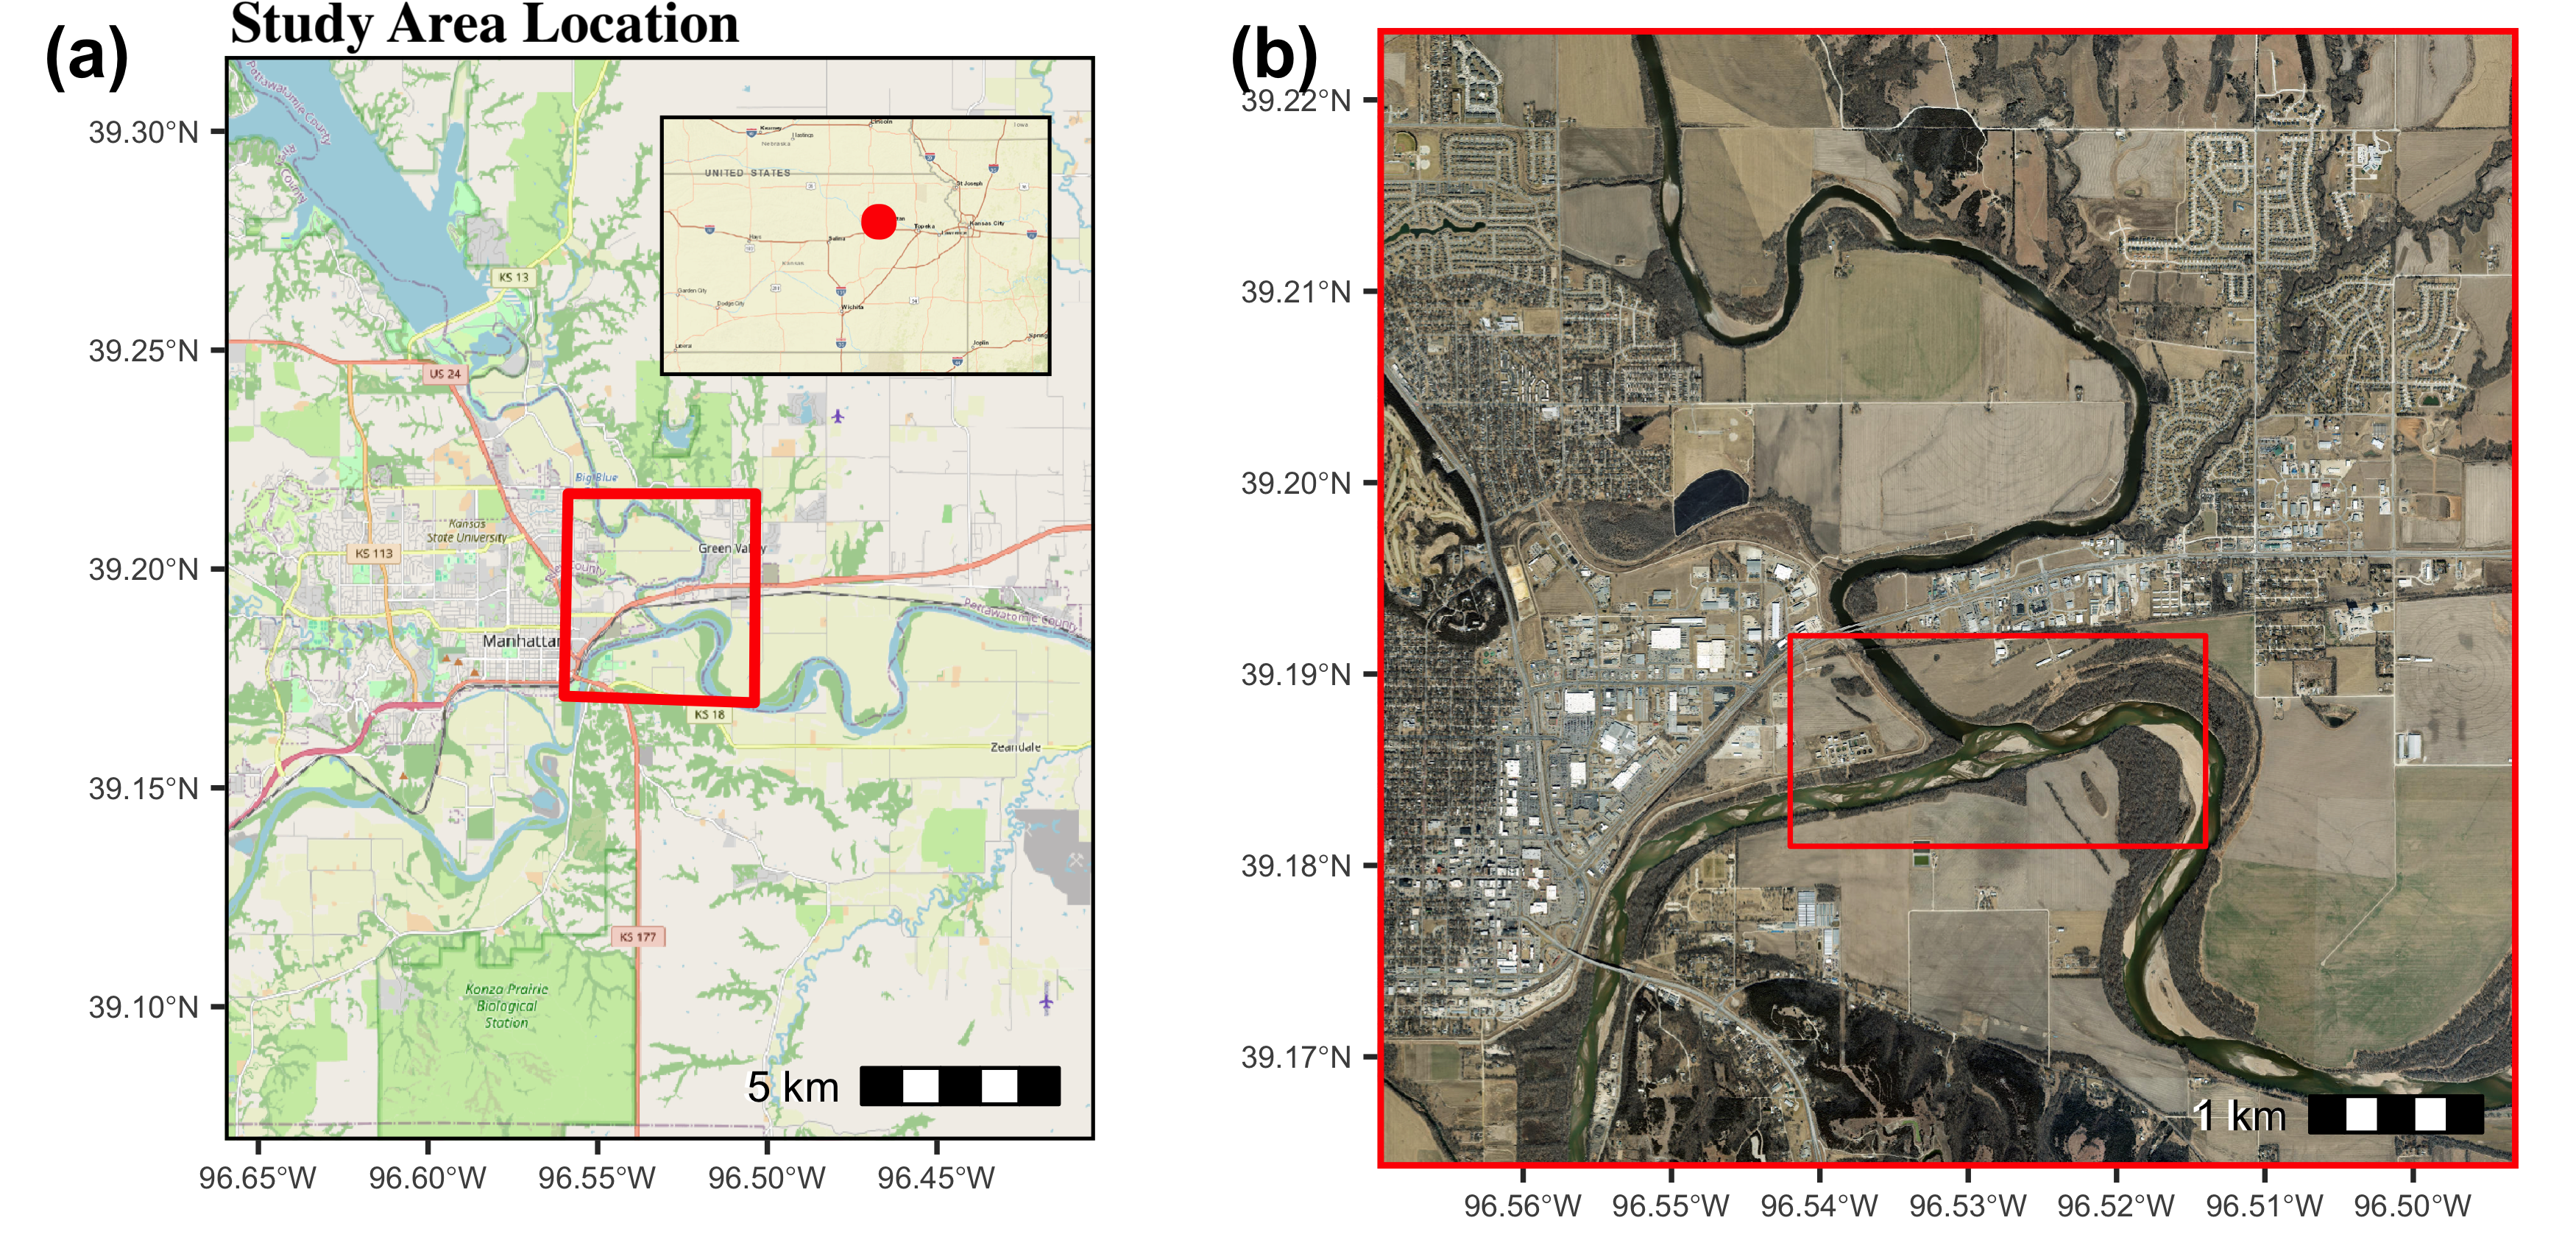
\includegraphics[width=0.99\linewidth]{fig1} 

}

\caption{The red square in left panel (a) represents the study area (b) which is adjacent to the city of Manhattan, Kansas, located roughly 200 kilometers west of Kansas City Metropolitan Area, United States (see inset map of (a)). The red square in the right panel (b) represents the location of the zoomed in portion of the subsequent figures.}\label{fig:studyArea}
\end{figure}

\subsection{Geospatial Preprocessing}\label{geospatial-preprocessing}

The area of interest (AOI) is located at the confluence of the Big Blue
and Kansas Rivers in the greater Manhattan, Kansas Area (Fig.
\ref{fig:studyArea}). The analysis domain was restricted to the river
corridor by applying a 30-m (98.4252-ft) buffer to the USGS Watershed
Boundary Dataset's (WBD) waterbody layer (USGS, 2023d). The river
corridor was later manually adjusted to include pointbars and other
portions of the river corridor that were beyond the buffer area from the
WBD. Because of the low resolution of the raster data, tributaries were
excluded from the analysis.

Landsat-9 (30-m) satellite images collected between November 21st, 2021
and November 14th, 2023 were retrieved via GEE (USGS, 2023c). Images
with more than 20\% cloud cover were excluded from the collection. In
total, there was a refined collection of 22 images covering all seasons
(Fig. \ref{fig:landsatBands}). The Landsat-9 imagery bands used for the
analysis contain seven bands including the coastal aerosol, blue, green,
red, near infrared (NIR), and two shortwave infrared (SWIR) bands (Fig.
\ref{fig:landsatBands}). Similarly, higher resolution (3-m) satellite
images from the same time period from the PS2, PS2.SD, and PSB.SD
satellites from the PlanetScope constellation were collected for the
same time period (Planet Labs PBC, 2024). Since the PlanetScope
inventory contained several snapshots of the AOI on a daily basis,
sometimes multiple times a day, only images with 0\% cloud cover were
included. The PlanetScope imagery was limited to the blue, green, red,
and NIR bands. The data for the 22 images were combined into two raster
stacks, one for Landsat and another for PlanetScope, with a combined
total of 154 and 88 bands respectively.

\begin{figure}

{\centering \includegraphics[width=0.99\linewidth]{fig2} 

}

\caption{Landsat-9 satellite image captured on 11-21-2021 and extracted from Google Earth Engine with each band displayed as a different sensor. The legend values indicate normalized surface reflectance (unitless).}\label{fig:landsatBands}
\end{figure}

\subsubsection{Aquatic Mesohabitat Types and Surface-Water Baseline
Distribution}\label{aquatic-mesohabitat-types-and-surface-water-baseline-distribution}

Aquatic mesohabitat types were defined from a 2D HEC-RAS simulation on a
3-m grid using depth--velocity thresholds consistent with mesoscale
typologies (Aadland, 1993; Wiest et al., 2024). Classes comprised (1)
shallow pool, (2) medium pool, (3) deep pool, (4) fast riffle, and (5)
raceway, (6) faster than a raceway, and (7) faster than a deep pool.
Seven hydrologic snapshots spanning the site's discharge regime were
selected from USGS mean-daily flow records via the \emph{dataRetrieval}
package (De Cicco et al., 2023): 2021-12-22 and 2022-02-12, 2022-04-17,
2022-05-31, 2022-06-20, 2022-07-18, and 2022-09-28 (Fig.
\ref{fig:usgsdata}).

\begin{figure}

{\centering \includegraphics[width=0.95\linewidth]{fig3} 

}

\caption{(a) Stream gauge data from three USGS sites (Fort Riley No.6879100, Wamego No.6887500, Manhattan No.6887000) near the study area, outlined in red, were used to identify seven dates with diverse flow conditions (filled circles in [b]). (b) Mean daily stream flow (cubic-ft/s), lines colored by site No.}\label{fig:usgsdata}
\end{figure}

\subsection{Semi-Supervised
Classification}\label{semi-supervised-classification}

A semi-supervised classification approach was used to categorize the
imagery into five classes: urban, bare land, non-forest vegetation,
forested land, and surface water. This ensemble approach involved
clustering the data into unsupervised classes using a K-means approach
and then classifying unseen data based off the new classes using a
supervised K-Nearest Neighbors (KNN) approach. The Hartigan-Wong K-means
algorithm was chosen to classify the image, which seeks the local optima
by shifting points from one cluster to another to assign the point to
the cluster with the smallest within-cluster sum of squares (Hartigan
and Wong, 1979).

Transitioning from unsupervised to supervised learning, KNN is
introduced as the classification algorithm. KNN is inherently simple yet
effective: for a given new instance, it identifies K nearest data points
based on a distance metric (e.g.~Euclidean distance) and assigns the new
instance to the most common class among its K nearest neighbors. The
integration of K-means clustering and KNN allowed us to utilize the
structure discovered in unlabeled data to classify new data points. The
assumption here is that the clusters formed during the K-means phase are
meaningful and represent different categories that can be used for
classification.

\subsection{Supervised Classification}\label{supervised-classification}

A supervised approach was used to classify pixels into five general
classes - bare land , non-forest vegetation (i.e.~shrubby, scattered
brush, or grasslands, etc.), forest, urban, and water based off the
Anderson land cover classification (Anderson et al., 1976). Land cover
classes were manually delineated within the AOI, each assigned one of
the classes using QGIS (QGIS Development Team, 2024). Only pixels that
remained unchanged within the study period were delineated to reduce the
variation between dates.

Training for a random forest classification model was performed on 80\%
of the class delineated pixels. The number of trees was set to 1000.
Model tuning parameters were ascertained via testing different
configurations on a five-fold cross-validation resampling of the
training data at 50m resolution. The highest accuracy and Receiver
Operating Characteristic Area Under the Curve (ROC AUC) were used as
indicators for picking the best modeling parameters. Two parameters were
tested: (1) minimum n, identified as the minimum number of data points
in a node that are required for the node to be split further, and (2)
the number of predictors that will be randomly sampled at each split
when creating the tree models.

The trained random forest model was used to predict the pixels across
the AOI for the raster stacks, creating a classified raster representing
the average conditions within the two-year period of image collection.
Additional, individual random forest models using the same model
parameters were produced and applied to the image pixels to create a
classified raster corresponding to each date.

\subsection{Time Series Analysis}\label{time-series-analysis}

The ML-classified rasters were masked to the river corridor to limit the
noise in the results. The average cell size was converted to acres
(1m\(^2\) = 0.00024711 acres) and was multiplied by the total number of
observations to estimate the total area per class. Two differencing
techniques were implemented to detect temporal change:
(\ref{eq:change_1}) difference in total area between an image date and
the following image date was calculated by subtracting the area by the
lag-one area and (\ref{eq:change_2}) the difference between the image
date and the baseline condition raster using the following set of
equations:

\begin{equation}\label{eq:change_1}
  area_{\delta1} = \sum_{i=1}^n area_{t_n} - \sum_{i=1}^n area_{t_{n+1}},
\end{equation}

\begin{equation}\label{eq:change_2}
  area_{\delta2} = \sum_{i=1}^n area_{t_0} - \sum_{i=1}^n area_{t_n},
\end{equation}

\noindent Where \(area\) is the total area, \(area_{\delta1}\) is the
temporal change in total area between consecutive dates,
\(area_{\delta2}\) is the change relative to the baseline condition,
\(t_0\) is the baseline condition, \(t_n\) represents a sampling date,
and \(t_{n+1}\) is the following sampling date.

\subsection{Model Evaluation}\label{model-evaluation}

\subsubsection{Comparison Analysis}\label{comparison-analysis}

To evaluate whether mesohabitat types can be predicted directly from
satellite data, rather than inferring inundation, HEC-RAS--derived
mesohabitat maps (Aadland, 1993; Wiest et al., 2024) were used as
categorical ground truth, and image-based models were trained to predict
eight classes: Shallow Pool, Med Pool, Deep Pool, Fast Riffle, Raceway,
Faster than a Raceway, and Faster than a Deep Pool. PlanetScope imagery
for each date was co-registered to the mesohabitat grid, and three
indices were derived from the four bands: Normalized Difference
Vegetation Index (NDVI), Normalized Difference Water Index (NDWI), and a
SWIR-free normalized burn-ratio (NBR) proxy suitable for sensors without
SWIR (e.g., PlanetScope).

\begin{equation}\label{eq:ndvi}
  NDVI = \frac{NIR - Red}{NIR + Red}
\end{equation}

\(NDVI\) highlights vegetation; values near +1 indicate dense green
cover.

\begin{equation}\label{eq:ndwi}
  NDWI = \frac{Green - NIR}{Green + NIR}
\end{equation}

\(NDWI\) enhances open-water detection via Green--NIR contrast.

\begin{equation}\label{eq:nbrb}
  NBR_{b} = \frac{NIR - Blue}{NIR + Blue}
\end{equation}

\(NBR_b\) is a SWIR-free analogue of the NBR, responsive to
moisture/substrate changes.

These indices were used as spectral predictors to train the mesohabitat
classification models. Predictors were restricted to PlanetScope because
it was the only sensor providing consistent, near--same-day coverage for
all seven hydraulic-model dates at this site, yielding a complete,
largely cloud-free stack aligned to the mesohabitat observations.
Landsat-9 imagery exhibited gaps and cloud contamination on several
target dates and introduced mixed-pixel issues for narrow channel
features; inclusion would have necessitated dropping dates or resampling
labels inconsistently. To reduce computation and harmonize supports,
PlantScope rasters were aggregated by a factor of five (spectral bands
averaged; mesohabitat labels aggregated by modal vote), yielding a
working cell size of \textasciitilde15 m.

A leave-one-date-out (LOO) design was adopted to respect the
flow-dependence of mesohabitats: for each held-out date (Dec 22 2021;
Feb 12, Apr 17, May 31, Jun 20, Jul 18, and Sep 28 2022), models were
trained on the remaining six dates and evaluated on the hold-out. Two
modeling approaches were compared:

\begin{enumerate}
\def\labelenumi{\arabic{enumi}.}
\item
  \textbf{Semi-supervised clustering:} Features were standardized;
  K-means was fit on training pixels (k = 12; nstart = 10). Each cluster
  was assigned a mesohabitat label by majority vote over training
  labels. The held-out date was predicted by nearest-center assignment
  in the standardized space.
\item
  \textbf{Supervised random forest:} A class-weighted random forest (800
  trees, mtry \(\le\) 6, min\_n = 5) was implemented via the R
  tidymodels/ranger packages. Class weights were set inversely
  proportional to class frequency in the training fold to mitigate
  imbalance. Predictors comprised the four bands plus the three indices.
\end{enumerate}

All modeling and evaluation were restricted to the mesohabitat mask
(i.e.~the river corridor). Performance was summarized per fold using
overall accuracy and Cohen's kappa; prediction maps for each held-out
date were exported as categorical rasters.

\newpage

\section{Results}\label{results}

\subsection{Median Mesohabitat
Distribution}\label{median-mesohabitat-distribution}

For each snapshot, the hydraulic model produced a categorical
mesohabitat map. A surface-water baseline mask was then derived as the
per-pixel median mesohabitat state across the seven dates (Fig.
\ref{fig:mesohabitats}); pixels outside this median mesohabitat
distribution were treated as non-water. Cloud-free PlanetScope scenes
acquired on or near the same dates of mean-daily flow records (Fig.
\ref{fig:usgsdata}) were co-registered to the hydraulic grid, and model
performance for the water vs.~non-water task was evaluated using
confusion matrices against this baseline.

\begin{figure}

{\centering \includegraphics[width=0.99\linewidth]{fig4} 

}

\caption{Predicted distribution of mesohabitats within the study area between December 2021 and September 2022 (see study area figure for reference location). Left panel displays the median distribution of mesohabitat types, which in aggregation represents the distribution of surface water. Right panel displays the mesohabitat types predicted for three of the seven mesohabitat sampling dates: December 22nd, 2021 and February 25th, 2022, and April 4th, 2023.}\label{fig:mesohabitats}
\end{figure}

\subsection{Optimized Semi-Supervised
Clustering}\label{optimized-semi-supervised-clustering}

With consideration of the elbow method for finding the optimal k for the
K-means clustering, i.e., the number of clusters, it was determined that
k between two and 15 is ideal, which is still subjective (Fig.
\ref{fig:determinek}). A silhouette analysis provided a measure of the
similarity between an object and the objects in its own cluster versus
the other clusters. Six clusters produced the highest average silhouette
width and was therefore chosen as the optimal value of k (Fig.
\ref{fig:determinek}). The algorithm was allowed to converge at up to
500 iterations. The K-means model was applied to the entire image
collection to establish baseline condition during the study period. Each
cluster produced from the K-means model was treated as a distinct class
(vegetation, forest, water, and mixed/bare land {[}either bare land or
urban{]}) which were used to train the KNN model (Fig.
\ref{fig:modelVisual}).

\begin{figure}

{\centering \includegraphics[width=0.99\linewidth]{fig5} 

}

\caption{K-means cluster quality was reviewed using the (a) elbow and (b) silhouette methods for Landsat-9 versus PlanetScope satellite imagery. Points highlighted in red identify the location of the optimal k value chosen for the number of clusters.}\label{fig:determinek}
\end{figure}

\begin{figure}

{\centering \includegraphics[width=0.99\linewidth]{fig6} 

}

\caption{Predicted distribution of  landcover types (a) from the unsupervised and (b) supervised models zoomed into the confluence of the Big Blue and Kansas Rivers (see study area figure for reference location). Left panel displays the baseline/static distribution of landcover types. Right panel displays the landcover types predicted for three of the 22 sampling dates: November 21st, 2021, August 25th, 2022, and April 4th, 2023.}\label{fig:modelVisual}
\end{figure}

\subsection{Optimized Supervised Learning
Model}\label{optimized-supervised-learning-model}

Testing revealed that the highest parameter-specific AUCs
(\textgreater{} 0.9975) for the random forest models were achieved when
minimum n and number of predictors were in between one to 20 and two to
25, respectively (Fig. \ref{fig:rf_tuning}(a)). The highest AUC was
achieved when minimum n is set to seven and the number of predictors was
set to six, therefore, these values were implemented in the random
forest model (Fig. \ref{fig:rf_tuning}(b)).

\begin{figure}

{\centering \includegraphics[width=0.99\linewidth]{fig7} 

}

\caption{The random forest parameters including minimum number of data points in a node and the number of predictors randomly sampled at each split were tuned by testing several configurations of random forest models with 1000 trees. The "best" area under the curve (AUC) was used as the configuration for the random forest model. (a) The optimal parameter-specific AUCs (before the dashed line) were used to test variations of the optimal tuning parameters (b). The arrow represents the highest AUC achieved, representing the best tuning parameters for the data.}\label{fig:rf_tuning}
\end{figure}

\subsection{Model Summary and
Performance}\label{model-summary-and-performance}

\subsubsection{Surface Water Validation}\label{surface-water-validation}

In terms of detecting change in LULC type, there were five comparable
classes: urban, bare land , non-forest vegetation, forested land, and
surface water. There were several differences between the higher
resolution PlanetScope dataset and the lower resolution Landsat dataset.
Notably, the PlanetScope data produced less variable results than
Landsat data, except for forested land and surface water for the
semi-supervised and supervised ML models, respectively (Fig.
\ref{fig:timeseries}{[}a-b{]}). Across both datasets, the average bare
land area predicted by the semi-supervised model was consistently higher
than that predicted by the supervised model. For instance, in the
Landsat dataset, the semi-supervised model predicted 147.83 acres
compared to 55.53 acres by supervised model. Similarly, in the
PlanetScope dataset, the semi-supervised model predicted 102.25 acres,
while the supervised model estimated 91.59 acres (Table
\ref{tab:areaTotal}).

Overall within-class variation was generally low for the bare land and
water classes (Fig. \ref{fig:timeseries}{[}a-b{]}). Specifically, the
change in area over time and difference in area from baseline conditions
was less variable for bare land in the supervised model and water in the
semi-supervised model (Fig. \ref{fig:timeseries}{[}a-b{]}). For surface
water, the models produced comparable average predictions, with
semi-supervised model estimating 372.81 acres and 372.51 acres for
Landsat and Planet, respectively, and supervised model estimating more
than 70 acres less acreage (293.45 acres and 302.86 acres) (Table
\ref{tab:areaTotal}).

\begin{figure}

{\centering \includegraphics[width=1\linewidth]{fig8} 

}

\caption{Image difference, \( \text{area}_{\delta1} \),  measure calculated using the difference in area from one sampling date to the following date.}\label{fig:timeseries}
\end{figure}
\begin{figure}

{\centering \includegraphics[width=1\linewidth]{fig9} 

}

\caption{Image difference, \( \text{area}_{\delta2} \), measure calculated using the difference in area between the baseline conditions and the sampling date.}\label{fig:timeseries_baseline}
\end{figure}

In comparison, the semi-supervised model predicted \textasciitilde2.71
times the amount of bare land than the supervised model in the Landsat
dataset, but relatively similar predictions in the PlanetScope dataset
(Table \ref{tab:areaTotal}). Regardless of the source data, the
semi-supervised model predicted more than 1,300-1,500 and 1,500-1,600
acres of surface water and forested land, respectively, while the
supervised model predicted 2,000-2,500 acres non-forest vegetation
(Table \ref{tab:areaTotal}). There was roughly \textasciitilde2.5 times
acreage of urban land cover predicted from the Landsat derived
supervised model than the similar model derived from Planet. Both models
generated similarly conservative outputs for surface water (Table
\ref{tab:areaTotal}).

Due to the non-normality and limited data points, a Kendall's tau
correlation coefficient was computed to test the relationship between
the bare land and surface water landcover types. The results revealed
that changes in surface water and bare land were moderate negatively
correlated (-0.49 and -0.39 in the Landsat and PlanetScope datasets,
respectively) for the semi-supervised model (Figures
\ref{fig:timeseries}(a)-\ref{fig:timeseries_baseline}(a)). Positive
changes in surface water area led to negative changes in bare land , and
vice versa. Theoretically, this correlation is expected as the river
corridor alternates between submersion at higher flows and islands
exposure at low flows. Similar patterns were not discernable for the
supervised model, where Kendall's tau produced a weakly correlated
relationship (0.04 and 0.06 in the Landsat and PlanetScope datasets,
respectively) (Figures
\ref{fig:timeseries}(b)-\ref{fig:timeseries_baseline}(a)).

\begingroup\fontsize{8}{10}\selectfont

\begin{longtable}[t]{cccccc}
\caption{\label{tab:areaTotal}Summary of average and total area (acres) of bare land  and surface water predicted by the ML models.}\\
\toprule
\multicolumn{2}{c}{ } & \multicolumn{2}{c}{Landsat} & \multicolumn{2}{c}{Planet} \\
\cmidrule(l{3pt}r{3pt}){3-4} \cmidrule(l{3pt}r{3pt}){5-6}
Area & Class & Semi-Supervised & Supervised & Semi-Supervised & Supervised\\
\midrule
Average & water & 372.81 & 293.45 & 372.51 & 302.86\\
 & water & 8201.84 & 6455.95 & 8195.18 & \vphantom{1} 6663.02\\
\specialrule{.1pt}{0pt}{0pt}
Total & water & 372.81 & 293.45 & 372.51 & 302.86\\
 & water & 8201.84 & 6455.95 & 8195.18 & 6663.02\\
\specialrule{.1pt}{0pt}{0pt}\\
\bottomrule
\end{longtable}
\endgroup{}

A confusion matrix comparing the baseline surface-water condition
predicted by the unsupervised and supervised learning models (created
during the comparitive analysis) against the HEC-RAS-derived median
mesohabitat distribution showed that the semi-supervised model correctly
classified approximately 65 more acres of water relative to the
supervised model (Table \ref{tab:conftb}). The supervised model
performed slightly better at classifying non-water conditions (Table
\ref{tab:conftb}). Overall, the semi-supervised approach outperformed
the supervised model on all reported metrics, including an accuracy of
0.88 and a kappa value of 0.73 (Table \ref{tab:conftb_stats}).

\begingroup\fontsize{8}{10}\selectfont

\begin{longtable}[t]{cccc}
\caption{\label{tab:conftb}Confusion table of the predicted model versus observations of water for classified mesohabitats.}\\
\toprule
\multicolumn{2}{c}{ } & \multicolumn{2}{c}{Observed} \\
\cmidrule(l{3pt}r{3pt}){3-4}
Model & Prediction & not water & water\\
\midrule
Semi-Supervised & water & 12 & 292\\
Supervised & water & 1 & 225\\
\specialrule{.1pt}{0pt}{0pt}\\
Semi-Supervised & not water & 124 & 45\\
Supervised & not water & 135 & 113\\
\specialrule{.1pt}{0pt}{0pt}\\
\bottomrule
\end{longtable}
\endgroup{}

\begingroup\fontsize{8}{10}\selectfont

\begin{longtable}[t]{c>{\centering\arraybackslash}p{2.4em}>{\centering\arraybackslash}p{2.4em}>{\centering\arraybackslash}p{2.4em}>{\centering\arraybackslash}p{2.4em}>{\centering\arraybackslash}p{2.4em}>{\centering\arraybackslash}p{2.4em}>{\centering\arraybackslash}p{2.4em}>{\centering\arraybackslash}p{2.4em}>{\centering\arraybackslash}p{2.4em}>{\centering\arraybackslash}p{2.4em}>{\centering\arraybackslash}p{2.4em}>{\centering\arraybackslash}p{2.4em}>{\centering\arraybackslash}p{2.4em}}
\caption{\label{tab:conftb_stats}Performance metrics of the predicted model versus observations of surface water derived from classified mesohabitats.}\\
\toprule
Model & Acc & Kappa & Sens & Spec & Pos Pred Val & Neg Pred Val & Matthews Corr Coef & J-index & Bal Acc & Det Prev & Prec & Recall & F Meas\\
\midrule
Semi-Supervised & 0.88 & 0.73 & 0.91 & 0.87 & 0.73 & 0.96 & 0.73 & 0.78 & 0.89 & 0.36 & 0.73 & 0.91 & 0.81\\
Supervised & 0.76 & 0.53 & 0.99 & 0.67 & 0.55 & 1.00 & 0.60 & 0.66 & 0.83 & 0.52 & 0.55 & 0.99 & 0.70\\
\bottomrule
\end{longtable}
\endgroup{}

\subsubsection{Mesohabitat Label
Prediction}\label{mesohabitat-label-prediction}

The LOO evaluation across seven dates yielded mean (± SD) per-pixel
accuracy of 0.149 ± 0.06 for the semi-supervised model and 0.208 ± 0.083
for the supervised model; mean Cohen's kappa was -0.001 ± 0.026 and
0.026 ± 0.024, respectively (Tables \ref{tab:loo_fold_metrics},
\ref{tab:loo_summary}). Accuracies varied by date (semi-supervised
range: 0.052--0.218; supervised range: 0.084--0.352), reflecting
differences in class composition among folds (Table
\ref{tab:loo_fold_metrics}). Categorical prediction rasters were
generated for each held-out date (Fig. \ref{fig:meso_preds}; Tables
\ref{tab:loo_fold_metrics}, \ref{tab:loo_summary}).

\begin{table}
\centering
\caption{\label{tab:loo_fold_metrics}LOO per-fold mesohabitat classification performance.}
\centering
\fontsize{8}{10}\selectfont
\begin{tabular}[t]{lccc}
\toprule
Date & Model & Accuracy & Kappa\\
\midrule
2021-12-22 & Semi-Supervised & 0.209 & 0.006\\
 & Supervised & 0.198 & 0.049\\
\specialrule{.1pt}{0pt}{0pt}\\
2022-02-12 & Semi-Supervised & 0.181 & -0.021\\
 & Supervised & 0.265 & 0.058\\
\specialrule{.1pt}{0pt}{0pt}\\
2022-04-17 & Semi-Supervised & 0.116 & -0.005\\
 & Supervised & 0.352 & 0.045\\
\specialrule{.1pt}{0pt}{0pt}\\
2022-05-31 & Semi-Supervised & 0.052 & -0.007\\
 & Supervised & 0.084 & -0.006\\
\specialrule{.1pt}{0pt}{0pt}\\
2022-06-20 & Semi-Supervised & 0.158 & 0.024\\
 & Supervised & 0.209 & 0.016\\
\specialrule{.1pt}{0pt}{0pt}\\
2022-07-18 & Semi-Supervised & 0.112 & 0.036\\
 & Supervised & 0.175 & 0.011\\
\specialrule{.1pt}{0pt}{0pt}\\
2022-09-28 & Semi-Supervised & 0.218 & -0.040\\
 & Supervised & 0.175 & 0.012\\
\specialrule{.1pt}{0pt}{0pt}\\
\bottomrule
\end{tabular}
\end{table}

\begin{table}
\centering
\caption{\label{tab:loo_summary}Cross-date summary (mean ± SD and range) of per-pixel performance across seven held-out dates.}
\centering
\fontsize{8}{10}\selectfont
\begin{tabular}[t]{lcccl}
\toprule
Model & Metric & Mean & SD & Range\\
\midrule
Semi-Supervised & Accuracy & 0.149 & 0.060 & 0.052–0.218\\
 & Kappa & -0.001 & 0.026 & -0.040–0.036\\
\specialrule{.1pt}{0pt}{0pt}\\
Supervised & Accuracy & 0.208 & 0.083 & 0.084–0.352\\
 & Kappa & 0.026 & 0.024 & -0.006–0.058\\
\specialrule{.1pt}{0pt}{0pt}\\
\bottomrule
\end{tabular}
\end{table}

\begin{landscape}

\begin{figure}

{\centering \includegraphics[width=1\linewidth]{fig10} 

}

\caption{Mesohabitat maps across seven dates at the Big Blue–Kansas River confluence. (a) Observed mesohabitat labels from the HEC-RAS–derived hydraulic model (Shallow Pool, Med Pool, Deep Pool, Fast Riffle, Raceway, Faster-than-a-Raceway, Faster-than-a-Deep-Pool).(b) Supervised (Random Forest; “Supervised”) image-based predictions from PlanetScope features (blue, green, red, NIR plus NDVI, NDWI, and NBR). (c) Semi-supervised (K-means plus majority label) image-based predictions from the same PlanetScope feature set. Facets are individual acquisition/model dates, ordered chronologically; all rasters are co-registered to the mesohabitat grid and aggregated to ~15 m for display. Colors are consistent across rows and correspond to the eight classes noted in the legend.}\label{fig:meso_preds}
\end{figure}

\end{landscape}

\newpage

\section{Discussion}\label{discussion}

\subsection{Summary of Principal
Findings}\label{summary-of-principal-findings}

Two complementary targets were evaluated. First, inundation (water
vs.~non-water) within the river corridor was recovered with high
agreement using the semi-supervised pipeline (accuracy = 0.88; k =
0.73), exceeding the supervised baseline (Table \ref{tab:conftb_stats};
Fig. \ref{fig:modelVisual}). This indicates strong and temporally stable
spectral separability of open water at the working scale, consistent
with the efficacy of visible--NIR contrasts and water indices for
surface-water mapping (Jin et al., 2021). Second, direct prediction of
mesohabitat labels (Shallow/Med/Deep Pool; Slow/Fast Riffle; Raceway;
Faster-than-a-Raceway; Faster-than-a-Deep-Pool) using a
leave-one-date-out design yielded modest cross-date performance (mean
per-pixel accuracy ≈ 0.20--0.21; mean k ≈ 0.02), with substantial
fold-to-fold variability linked to class composition and discharge state
(Tables \ref{tab:loo_fold_metrics}, \ref{tab:loo_summary}). Despite low
absolute metrics, prediction maps show coherent spatial structure (e.g.,
pool-like classes along the thalweg; high-velocity classes near
constrictions; Fig. \ref{fig:meso_preds}), indicating a learnable signal
from four-band PlanetScope features even after aggregation.

\subsubsection{Interpretation of Inundation
Results}\label{interpretation-of-inundation-results}

The semi-supervised pipeline yielded six clusters that were readily
consolidated into five land-cover labels. Within the river corridor,
impervious and bare substrates were not reliably separable spectrally;
treating mixed/impervious pixels as ``bare land'' was appropriate given
the absence of in-channel infrastructure aside from static bridge decks,
which do not affect temporal comparisons. Choice of the cluster count
(k) remains subjective and was fixed for consistency; a formal
sensitivity analysis (varying k, band sets, and date combinations) was
not undertaken here but would clarify stability versus over-partitioning
trade-offs under noisy conditions (Vahidi et al., 2023).

Across sensors, the semi-supervised change signal was comparatively
insensitive to input resolution. PlanetScope at \textasciitilde3 m
captured finer temporal variation in areal change, as expected, yet
Landsat-9 at 30 m produced change patterns that were directionally
consistent and of similar magnitude. This concordance indicates that
rapid, lower-resolution deployments can recover robust mesoscale trends,
while higher-resolution inputs refine the amplitude and spatial detail
of detected changes.

\subsubsection{Interpretation of Mesohabitat
Results}\label{interpretation-of-mesohabitat-results}

Given mean per-pixel accuracies of 0.149 (semi-supervised) and 0.208
(supervised) with mean Cohen's kappa of -0.001 and 0.026, respectively
(Tables \ref{tab:loo_fold_metrics}, \ref{tab:loo_summary}), direct
mesohabitat classification from four-band PlanetScope features at the
aggregated support performs at or only slightly above chance, with the
semi-supervised variant occasionally below chance. This outcome is
consistent with several interacting factors. First, class boundaries are
flow-dependent and nonstationary: mesohabitats translate, expand, and
contract with discharge and local hydraulics, so a given pixel can
change label across dates, penalizing cross-date generalization unless
hydrodynamic context is encoded Harris et al. (2024). Second,
aggregation to \textasciitilde15 m introduces sub-pixel mixing in narrow
channels and along riffle pool transitions, attenuating spectral
contrast and blurring boundaries. Third, several mesohabitat
distinctions are spectrally ambiguous at four bands because they are
partly morphodynamic states; much of their separability is carried by
surface-texture and morphological cues (e.g., roughness patterns, local
slope/curvature) not modeled here Moortgat et al. (2022). Class
imbalance further limits parameter learning; some classes are sparse or
absent in particular folds---even with inverse-frequency weighting Ma et
al. (2019). Finally, label noise from model such that image mismatch
(e.g.~minor timing offsets between imagery and hydraulics, bathymetric
uncertainty, co-registration drift) propagates into the categorical
targets and caps attainable kappa under stringent cross-date validation.
Under these constraints, near-zero, and occasionally negative kappa
values are expected at the aggregated grain with a purely spectral
feature set; nonetheless, qualitative spatial coherence in predicted
maps suggests partial signal that could be amplified by adding texture
and morphological context.

\subsection{Sources of Error and
Uncertainty}\label{sources-of-error-and-uncertainty}

Three error modes were most evident: (i) edge confusion at unit
boundaries where mixed pixels dominate; (ii) systematic bias toward
dominant classes in the semi-supervised cluster-to-label step when
clusters straddle multiple units; and (iii) fold-specific shocks when
rare classes vanish from training or test, producing unstable per-fold k
These behaviors mirror sensitivities reported in object- and pixel-based
riverscape mapping where segmentation parameters, illumination, and
turbidity modulate separability (Demarchi et al., 2016a; Kutz et al.,
2022; Zhang et al., 2023). Uncertainty quantification (e.g., entropy of
class probabilities) was not computed here but is recommended to flag
ambiguous zones for analyst review.

\subsection{Practical implications}\label{practical-implications}

From a monitoring standpoint, the inundation pipeline is
deployment-ready for tracking wetted area and corridor dynamics through
time. The mesohabitat pipeline should be treated as proof-of-concept: it
reveals where image-only predictors already align with hydraulic classes
and where additional information is required to meet decision thresholds
(e.g., habitat suitability modeling, restoration design). Importantly,
the results support a tiered product strategy: use surface water maps
operationally and generate mesohabitat layers where data richness
permits.

\subsection{Future considerations}\label{future-considerations}

Targeted enhancements are expected to materially improve mesohabitat
accuracy and kappa:

\begin{itemize}
\tightlist
\item
  Restore native spatial support (\textasciitilde3 m) and add texture
  metrics (e.g., Gray-Level Co-occurrence Matrix {[}GLCM{]} contrast,
  entropy, local variance) to encode surface roughness and flow
  streaking (Farwell et al., 2021).
\item
  Incorporate morphological context from DEM-derived slope/curvature or
  shallow bathymetry proxies where available, aligning with evidence
  that OBIA/terrain fusion improves riverscape unit mapping (Demarchi et
  al., 2016a).
\item
  Adopt a hierarchical classifier (i.e.~water to unit family to
  subclass) to reduce confusability among fine classes and stabilize
  minority categories.
\item
  Explore spatial models (e.g., shallow CNN on PlanetScope tiles or RF
  with engineered texture windows) to inject neighborhood context beyond
  pixel spectra (Ma et al., 2019; Moortgat et al., 2022).
\item
  Use cost-sensitive learning and focal sampling for rare classes;
  consider active learning to prioritize annotation where uncertainty is
  high (Maskey et al., 2018).
\item
  Where feasible, evaluate hybrid/physics-informed fusion that brings
  co-registered hydraulic predictors (i.e.~depth/velocity rasters)
  alongside imagery, an approach likely to raise ceiling performance
  (Harris et al., 2024).
\item
  Quantify predictive uncertainty (e.g.~calibration), enabling
  conservative products for management use.
\end{itemize}

\subsection{Conclusion}\label{conclusion}

Satellite-based workflows accurately recover inundation within river
corridors and offer a scalable foundation for riverscape monitoring.
Direct mesohabitat prediction from four-band PlanetScope features at
aggregated resolution yields modest cross-date accuracy but exhibits
meaningful spatial structure, indicating that mesohabitat signal is
present and partially learnable. The path to decision-grade products is
clear: use fine spatial resolution where possible, enrich features with
texture and morphology, adopt hierarchical/imbalance-aware learning,
and, where available, fuse hydraulics. Together, these steps align with
the broader trajectory in high-resolution RS and ecohydraulics toward
routine, basin-scale mapping of mesoscale habitat structure (Moortgat et
al., 2022; Verma et al., 2021; Wegscheider et al., 2020).

\subsubsection*{Author Contributions}\label{author-contributions}
\addcontentsline{toc}{subsubsection}{Author Contributions}

\textbf{E.C.}: conceptualization, methodology, software, formal
analysis, investigation, data management, writing - original and draft,
visualization, funding acquisition. \textbf{A.H.}: conceptualization,
supervision, validation and QAQC, review and editing, resources, writing
- review and editing, funding acquisition, and project administration.

\subsubsection*{Funding}\label{funding}
\addcontentsline{toc}{subsubsection}{Funding}

The project was funded by the US Army Corps of Engineers' (USACE)
Aquatic and Nuisance Species Research Program focus on Next Generation
Ecological Modeling. This research was supported in part by an
appointment to the Department of Defense (DOD) Research Participation
Program administered by the Oak Ridge Institute for Science and
Education (ORISE) through an interagency agreement between the U.S.
Department of Energy (DOE) and the DOD. ORISE is managed by ORAU under
DOE contract number DE-SC0014664. All opinions expressed in this paper
are the author's and do not necessarily reflect the policies and views
of DOD, DOE, or ORAU/ORISE.

\subsubsection*{Acknowledgements}\label{acknowledgements}
\addcontentsline{toc}{subsubsection}{Acknowledgements}

\textbf{E.C.} gratefully acknowledges the Environmental Laboratory of
the USACE Engineer Research and Development Center (ERDC) and
\textbf{A.H.} for funding, data access, and technical support that
enabled this research. \textbf{E.C.} also acknowledges the Department of
Marine Sciences at the University of Puerto Rico--Mayagüez for
logistical and academic support during graduate research and
dissertation-related activities.

\subsubsection*{Conflict of Interest}\label{conflict-of-interest}
\addcontentsline{toc}{subsubsection}{Conflict of Interest}

The authors declare no competing interests.

\subsubsection*{Availability of data and
materials}\label{availability-of-data-and-materials}
\addcontentsline{toc}{subsubsection}{Availability of data and materials}

The stream discharge data were retrieved from the USGS (De Cicco et al.,
2023). The 30-m Landsat-9 satellite imagery can be retrieved from the
USGS Landsat Collection (USGS, 2023c). The 3-m PlanetScope satellite
imagery was accessed under a research license provided by Planet Labs
(Planet Labs PBC, 2024), enabling the use of the data for academic
purposes. The data that support the findings of this study are available
from the corresponding author upon reasonable request. The river
corridor shapefile and R code used for this analysis has been uploaded
to Github and made publicly available via a General Public Use License.
The repository can be accessed with the following link:
\url{<https://github.com/el-cordero/meso-change.git>}

\newpage

\section*{References}\label{references}
\addcontentsline{toc}{section}{References}

\singlespacing

\phantomsection\label{refs}
\begin{CSLReferences}{1}{0}
\bibitem[\citeproctext]{ref-aadlandStreamHabitatTypes1993}
Aadland, L., 1993. Stream {Habitat Types}: {Their Fish Assemblages} and
{Relationship} to {Flow}. North American Journal of Fisheries Management
13, 790--806.
\url{https://doi.org/10.1577/1548-8675(1993)013\%3C0790:SHTTFA\%3E2.3.CO;2}

\bibitem[\citeproctext]{ref-aggarwalNeuralNetworksDeep2018}
Aggarwal, C.C., 2018. Neural {Networks} and {Deep Learning}: {A
Textbook}. Springer International Publishing, Cham.
\url{https://doi.org/10.1007/978-3-319-94463-0}

\bibitem[\citeproctext]{ref-andersonLandUseLand1976}
Anderson, J.R., Hardy, E.E., Roach, J.T., Witmer, R.E., 1976. A {Land
Use} and {Land Cover Classification System} for {Use} with {Remote
Sensor Data} (No. 964). United States Geological Survey.

\bibitem[\citeproctext]{ref-aybarCombiningReeInBook}
Aybar, C., Loaiza, D., Barja, A., Herrera, F., Gonzales, A., Espinoza,
W., 2024. Combining {R} and earth engine, in: Cardille, J.A., Crowley,
M.A., Saah, D., Clinton, N.E. (Eds.), Cloud-{Based Remote Sensing} with
{Google Earth Engine}. pp. 629--651.
\url{https://doi.org/10.1007/978-3-031-26588-4_31}

\bibitem[\citeproctext]{ref-aybarRgeePackageInteracting2020}
Aybar, C., Wu, Q., Bautista, L., Yali, R., Barja, A., 2020.
{\emph{Rgee}}: {An R} package for interacting with {Google Earth
Engine}. Journal of Open Source Software 5, 2272.
\url{https://doi.org/10.21105/joss.02272}

\bibitem[\citeproctext]{ref-brostowSemanticObjectClasses2009}
Brostow, G.J., Fauqueur, J., Cipolla, R., 2009. Semantic object classes
in video: {A} high-definition ground truth database. Pattern Recognition
Letters 30, 88--97. \url{https://doi.org/10.1016/j.patrec.2008.04.005}

\bibitem[\citeproctext]{ref-calderonInfluenceMesohabitatStructures2016}
Calderon, M.S., An, K.-G., 2016. An influence of mesohabitat structures
(pool, riffle, and run) and land-use pattern on the index of biological
integrity in the {Geum River} watershed. Journal of Ecology and
Environment 40, 13. \url{https://doi.org/10.1186/s41610-016-0018-8}

\bibitem[\citeproctext]{ref-cavender-baresIntegratingRemoteSensing2022}
Cavender-Bares, J., Schneider, F.D., Santos, M.J., Armstrong, A.,
Carnaval, A., Dahlin, K.M., Fatoyinbo, L., Hurtt, G.C., Schimel, D.,
Townsend, P.A., Ustin, S.L., Wang, Z., Wilson, A.M., 2022. Integrating
remote sensing with ecology and evolution to advance biodiversity
conservation. Nature Ecology \& Evolution 6, 506--519.
\url{https://doi.org/10.1038/s41559-022-01702-5}

\bibitem[\citeproctext]{ref-choukikerLiteratureReviewLand2021}
Choukiker, S.K., Dohare, D., 2021. A {Literature Review} on {Land Use
Land Cover Changes Detection} using {Remote Sensing} and {GIS}.
International Journal for Research in Applied Science and Engineering
Technology 9, 725--735.
\url{https://doi.org/10.22214/ijraset.2021.33349}

\bibitem[\citeproctext]{ref-deciccoDataRetrievalPackagesDiscovering2023}
De Cicco, L.A., Hirsch, R.M., Lorenz, D., Watkins, D., Johnson, M.,
2023. {\emph{dataRetrieval}}: {R} packages for discovering and
retrieving water data available from {U}.{S}. Federal hydrologic web
services. \url{https://doi.org/10.5066/P9X4L3GE}

\bibitem[\citeproctext]{ref-demarchiHierarchicalObjectBasedMapping2016}
Demarchi, L., Bizzi, S., Piégay, H., 2016a. Hierarchical {Object-Based
Mapping} of {Riverscape Units} and in-{Stream Mesohabitats Using LiDAR}
and {VHR Imagery}. Remote Sensing 8, 97.
\url{https://doi.org/10.3390/rs8020097}

\bibitem[\citeproctext]{ref-demarchiHierarchicalObjectBasedMapping2016a}
Demarchi, L., Bizzi, S., Piégay, H., 2016b. Hierarchical {Object-Based
Mapping} of {Riverscape Units} and in-{Stream Mesohabitats Using LiDAR}
and {VHR Imagery}. Remote Sensing 8, 97.
\url{https://doi.org/10.3390/rs8020097}

\bibitem[\citeproctext]{ref-demirDeepGlobe2018Challenge2018}
Demir, I., Koperski, K., Lindenbaum, D., Pang, G., Huang, J., Basu, S.,
Hughes, F., Tuia, D., Raskar, R., 2018. {DeepGlobe} 2018: {A Challenge}
to {Parse} the {Earth} through {Satellite Images}, in: 2018 {IEEE}/{CVF
Conference} on {Computer Vision} and {Pattern Recognition Workshops}
({CVPRW}). IEEE, Salt Lake City, UT, USA, pp. 172--17209.
\url{https://doi.org/10.1109/CVPRW.2018.00031}

\bibitem[\citeproctext]{ref-eltayebelmahalSpatialCloudComputing2023}
Eltayeb Elmahal, A., Mahmoud Ibrahim Musa, M., 2023. Spatial {Cloud
Computing Using Google Earth Engine} and {R Packages}, in: Geographic
{Information Systems} - {Data Science Approach} {[}{Working Title}{]}.
IntechOpen. \url{https://doi.org/10.5772/intechopen.1002686}

\bibitem[\citeproctext]{ref-farwellSatelliteImageTexture2021}
Farwell, L.S., Gudex-Cross, D., Anise, I.E., Bosch, M.J., Olah, A.M.,
Radeloff, V.C., Razenkova, E., Rogova, N., Silveira, E.M.O., Smith,
M.M., Pidgeon, A.M., 2021. Satellite image texture captures vegetation
heterogeneity and explains patterns of bird richness. Remote Sensing of
Environment 253, 112175. \url{https://doi.org/10.1016/j.rse.2020.112175}

\bibitem[\citeproctext]{ref-fixDiscriminatoryAnalysisNonparametric1989}
Fix, E., Hodges, J.L., 1989. Discriminatory {Analysis}. {Nonparametric
Discrimination}: {Consistency Properties}. International Statistical
Review / Revue Internationale de Statistique 57, 238.
\url{https://doi.org/10.2307/1403797}

\bibitem[\citeproctext]{ref-ganeshIntegrationGISMachine2023}
Ganesh, B., Vincent, S., Pathan, S., Benitez, S.R.G., 2023. Integration
of {GIS} and {Machine Learning Techniques} for {Mapping} the
{Landslide-Prone Areas} in the {State} of {Goa}, {India}. Journal of the
Indian Society of Remote Sensing 51, 1479--1491.
\url{https://doi.org/10.1007/s12524-023-01707-y}

\bibitem[\citeproctext]{ref-griffinUsingUnmannedAircraft2020}
Griffin, S., Lasko, J.C., 2020. Using {Unmanned Aircraft System} ({UAS})
and {Satellite Imagery} to {Map Aquatic} and {Terrestrial Vegetation}
(No. ERDC/GRL TN-20-4). {U.S. Army Engineer Research and Development
Center}, Vicksburg, MS. \url{https://doi.org/10.21236/ADA572123}

\bibitem[\citeproctext]{ref-harrisHydraulicAnalysisAssessing2024}
Harris, A., Porter, M., McKay, S.K., Mulchandani, A., Stone, M., 2024.
Hydraulic analysis for assessing environmental flow selection and
ecological model formulation. Ecohydrology 17, e2681.
\url{https://doi.org/10.1002/eco.2681}

\bibitem[\citeproctext]{ref-hartiganAlgorithm136KMeans1979}
Hartigan, J.A., Wong, M.A., 1979. Algorithm {AS} 136: {A K-Means
Clustering Algorithm}. Applied Statistics 28, 100.
\url{https://doi.org/10.2307/2346830}

\bibitem[\citeproctext]{ref-hernangomezUsingTidyverseTerra2023}
Hernangómez, D., 2023. Using the tidyverse with terra objects: The
tidyterrapackage. Journal of Open Source Software 8, 5751.
\url{https://doi.org/10.21105/joss.05751}

\bibitem[\citeproctext]{ref-hijmansTerraSpatialData2024}
Hijmans, R.J., 2024. {\emph{Terra}}: {Spatial Data Analysis}.

\bibitem[\citeproctext]{ref-howardDeepLearningCoders2020}
Howard, J., Gugger, S., 2020. Deep learning for coders with fastai and
{PyTorch}: {AI} applications without a {PhD}, First edition. ed.
O'Reilly, Beijing Boston Farnham Sebastopol Tokyo.

\bibitem[\citeproctext]{ref-jinRiverBodyExtraction2021}
Jin, S., Liu, Y., Fagherazzi, S., Mi, H., Qiao, G., Xu, W., Sun, C.,
Liu, Y., Zhao, B., Fichot, C.G., 2021. River body extraction from
sentinel-{2A}/{B MSI} images based on an adaptive multi-scale region
growth method. Remote Sensing of Environment 255, 112297.
\url{https://doi.org/10.1016/j.rse.2021.112297}

\bibitem[\citeproctext]{ref-johansenUsingUnmannedAircraft2022}
Johansen, R.A., Reif, M.K., Saltus, C.L., Pokrzywinski, K.L., 2022.
Using {Unmanned Aircraft System} ({UAS}) and {Satellite Imagery} to {Map
Aquatic} and {Terrestrial Vegetation} (No. ERDC/EL SR-22-2). {U.S. Army
Engineer Research and Development Center Environmental Laboratory},
Vicksburg, MS. \url{https://doi.org/10.21236/ADA572123}

\bibitem[\citeproctext]{ref-kuhnBuildingPredictiveModels2008}
Kuhn, M., 2008. Building predictive models in {R} using the caret
package. Journal of Statistical Software 28, 1--26.
\url{https://doi.org/10.18637/jss.v028.i05}

\bibitem[\citeproctext]{ref-kuhnTidymodelsCollectionPackages2020}
Kuhn, M., Wickham, H., 2020. Tidymodels: A collection of packages for
modeling and machine learning using tidyverse principles.

\bibitem[\citeproctext]{ref-kutzObjectBasedClassification2022}
Kutz, K., Cook, Z., Linderman, M., 2022. Object based classification of
a riparian environment using ultra-high resolution imagery, hierarchical
landcover structures, and image texture. Scientific Reports 12, 11291.
\url{https://doi.org/10.1038/s41598-022-14757-y}

\bibitem[\citeproctext]{ref-lantzMachineLearning2023}
Lantz, B., 2023. Machine {Learning} with {R}, Fourth. ed. Packt
Publishing Ltd, Birmingham, U.K.

\bibitem[\citeproctext]{ref-liDeepLearningRemote2018}
Li, Y., Zhang, H., Xue, X., Jiang, Y., Shen, Q., 2018. Deep learning for
remote sensing image classification: {A} survey. WIREs Data Mining and
Knowledge Discovery 8, e1264. \url{https://doi.org/10.1002/widm.1264}

\bibitem[\citeproctext]{ref-limChangeDetectionHigh2018}
Lim, K., Jin, D., Kim, C.-S., 2018. Change {Detection} in {High
Resolution Satellite Images Using} an {Ensemble} of {Convolutional
Neural Networks}, in: 2018 {Asia-Pacific Signal} and {Information
Processing Association Annual Summit} and {Conference} ({APSIPA ASC}).
IEEE, Honolulu, HI, USA, pp. 509--515.
\url{https://doi.org/10.23919/APSIPA.2018.8659603}

\bibitem[\citeproctext]{ref-lindenschmidtGeospatialModelingRiver2018}
Lindenschmidt, K.-E., Carr, M., 2018. Geospatial {Modeling} of {River
Systems}. Water 10, 282. \url{https://doi.org/10.3390/w10030282}

\bibitem[\citeproctext]{ref-maDeepLearningRemote2019}
Ma, L., Liu, Y., Zhang, X., Ye, Y., Yin, G., Johnson, B.A., 2019. Deep
learning in remote sensing applications: {A} meta-analysis and review.
ISPRS Journal of Photogrammetry and Remote Sensing 152, 166--177.
\url{https://doi.org/10.1016/j.isprsjprs.2019.04.015}

\bibitem[\citeproctext]{ref-mandlikReviewRemoteSensing2018a}
Mandlik, G.G., Mundhe, R.N., 2018. A {Review} of {Remote Sensing
Techniques For Land Use Land Cover Change Detection Techniques}. Journal
of Emerging Technologies and Innovative Research 5, 900--902.

\bibitem[\citeproctext]{ref-marcusRemoteSensingRivers2010}
Marcus, W.A., Fonstad, M.A., 2010. Remote sensing of rivers: The
emergence of a subdiscipline in the river sciences. Earth Surface
Processes and Landforms 35, 1867--1872.
\url{https://doi.org/10.1002/esp.2094}

\bibitem[\citeproctext]{ref-maskeyEarthScienceDeep2018}
Maskey, M., Ramachandran, R., Miller, J.J., Zhang, J., Gurung, I., 2018.
Earth {Science Deep Learning}: {Applications} and {Lessons Learned}, in:
{IGARSS} 2018 - 2018 {IEEE International Geoscience} and {Remote Sensing
Symposium}. IEEE, Valencia, pp. 1760--1763.
\url{https://doi.org/10.1109/IGARSS.2018.8517346}

\bibitem[\citeproctext]{ref-mckayNewYorkBight2022}
McKay, S.K., Mahan, V., Dougherty, M.P., Swannack, T.M., Hall, C.,
Saltus, C.L., Reif, M.K., Allen, S., 2022. New {York Bight Ecological
Model} ({NYBEM}), {Version} 1.0.0. USACE, Environmental Laboratory.

\bibitem[\citeproctext]{ref-moortgatDeepLearningModels2022}
Moortgat, J., Li, Z., Durand, M., Howat, I., Yadav, B., Dai, C., 2022.
Deep learning models for river classification at sub-meter resolutions
from multispectral and panchromatic commercial satellite imagery. Remote
Sensing of Environment 282, 113279.
\url{https://doi.org/10.1016/j.rse.2022.113279}

\bibitem[\citeproctext]{ref-niedballaImagesegPackageDeep2022}
Niedballa, J., Axtner, J., Döbert, T.F., Tilker, A., Nguyen, A., Wong,
S.T., Fiderer, C., Heurich, M., Wilting, A., 2022. Imageseg: {An R}
package for deep learning-based image segmentation. Methods in Ecology
and Evolution 13, 2363--2371.
\url{https://doi.org/10.1111/2041-210X.13984}

\bibitem[\citeproctext]{ref-planetlabspbcPlanetApplicationProgram2024}
Planet Labs PBC, 2024. Planet application program interface: {In} space
for life on earth.

\bibitem[\citeproctext]{ref-qgisdevelopmentteamQGISGeographicInformation2024}
QGIS Development Team, 2024. {QGIS Geographic Information System}.

\bibitem[\citeproctext]{ref-rcoreteamLanguageEnvironmentStatistical2023}
R Core Team, 2023. {\emph{R}}: {A} language and environment for
statistical computing.

\bibitem[\citeproctext]{ref-romeroUnsupervisedDeepFeature2016}
Romero, A., Gatta, C., Camps-Valls, G., 2016. Unsupervised {Deep Feature
Extraction} for {Remote Sensing Image Classification}. IEEE Transactions
on Geoscience and Remote Sensing 54, 1349--1362.
\url{https://doi.org/10.1109/TGRS.2015.2478379}

\bibitem[\citeproctext]{ref-schwartzUseEcohydraulicBasedMesohabitat2016}
Schwartz, J., 2016. Use of {Ecohydraulic-Based Mesohabitat
Classification} and {Fish Species Traits} for {Stream Restoration
Design}. Water 8, 520. \url{https://doi.org/10.3390/w8110520}

\bibitem[\citeproctext]{ref-shabatComparativeStudyUse2017}
Shabat, A.M., Tapamo, J.-R., 2017. A comparative study of the use of
local directional pattern for texture-based informal settlement
classification. Journal of Applied Research and Technology 15, 250--258.
\url{https://doi.org/10.1016/j.jart.2016.12.009}

\bibitem[\citeproctext]{ref-shashikantConvolutionalNeuralNetwork2019}
Shashikant, 2019. Convolutional {Neural Network}: {A Step By Step
Guide}. towards data science.

\bibitem[\citeproctext]{ref-suirMultiTemporalTrendAnalysis2023}
Suir, G.M., Jackson, S., Saltus, C., Reif, M., 2023. Multi-{Temporal
Trend Analysis} of {Coastal Vegetation Using Metrics Derived} from
{Hyperspectral} and {LiDAR Data}. Remote Sensing 15, 2098.
\url{https://doi.org/10.3390/rs15082098}

\bibitem[\citeproctext]{ref-suttidateEffectsHabitatHeterogeneity2023}
Suttidate, N., Pidgeon, A.M., Hobi, M.L., Round, P.D., Dubinin, M.,
Radeloff, V.C., 2023. The effects of habitat heterogeneity, as measured
by satellite image texture, on tropical forest bird distributions.
Biological Conservation 281, 110002.
\url{https://doi.org/10.1016/j.biocon.2023.110002}

\bibitem[\citeproctext]{ref-thompsonRealizingMachineLearnings2021}
Thompson, D., Brodrick, P., 2021. Realizing {Machine Learning}'s
{Promise} in {Geoscience Remote Sensing}. Eos 102.
\url{https://doi.org/10.1029/2021EO160605}

\bibitem[\citeproctext]{ref-usdaNationalAgricultureImagery}
USDA, n.d. National {Agriculture Imagery Program} ({NAIP}) {GeoHub}.

\bibitem[\citeproctext]{ref-usgsLandsatCollection2023}
USGS, 2023c. Landsat {Collection}.

\bibitem[\citeproctext]{ref-usgsUSGS1Meter2023}
USGS, 2023a. {USGS} 1 {Meter} 14 X71y435 {KS}\_{Statewide}\_2018\_{A18}.

\bibitem[\citeproctext]{ref-usgsUSGS1Meter2023a}
USGS, 2023b. {USGS} 1 {Meter} 14 X71y434 {KS}\_{Statewide}\_2018\_{A18}.

\bibitem[\citeproctext]{ref-usgsUSGSWatershedBoundary2023}
USGS, 2023d. {USGS Watershed Boundary Dataset} ({WBD}) for {Kansas}.

\bibitem[\citeproctext]{ref-usgsHighResolutionOrthoimagery2011}
USGS, 2011. High {Resolution Orthoimagery Manhattan-Riley Co},{KS}.

\bibitem[\citeproctext]{ref-vahidiOptimalBandSelection2023}
Vahidi, M., Aghakhani, S., Martín, D., Aminzadeh, H., Kaveh, M., 2023.
Optimal band selection using evolutionary machine learning to improve
the accuracy of hyper-spectral images classification: A novel
migration-based particle swarm optimization. Journal of Classification
40. \url{https://doi.org/10.1007/s00357-023-09448-w}

\bibitem[\citeproctext]{ref-vanrooijenSpatiotemporalDistributionRiver2024}
Van Rooijen, E., Lotsari, E., 2024. The spatiotemporal distribution of
river bank erosion events and their drivers in seasonally frozen
regions. Geomorphology 454, 109140.
\url{https://doi.org/10.1016/j.geomorph.2024.109140}

\bibitem[\citeproctext]{ref-vermaDeepRivWidthDeepLearning2021}
Verma, U., Chauhan, A., M. M., M.P., Pai, R., 2021. {DeepRivWidth} :
{Deep} learning based semantic segmentation approach for river
identification and width measurement in {SAR} images of {Coastal
Karnataka}. Computers \& Geosciences 154, 104805.
\url{https://doi.org/10.1016/j.cageo.2021.104805}

\bibitem[\citeproctext]{ref-wangDeprivationPocketsLens2019}
Wang, J., Kuffer, M., Roy, D., Pfeffer, K., 2019. Deprivation pockets
through the lens of convolutional neural networks. Remote Sensing of
Environment 234, 111448. \url{https://doi.org/10.1016/j.rse.2019.111448}

\bibitem[\citeproctext]{ref-wegscheiderMesohabitatModellingFish2020}
Wegscheider, B., Linnansaari, T., Curry, R.A., 2020. Mesohabitat
modelling in fish ecology: {A} global synthesis. Fish and Fisheries 21,
927--939. \url{https://doi.org/10.1111/faf.12477}

\bibitem[\citeproctext]{ref-wiestHydraulicModelHECRAS2024}
Wiest, S., Harris, A., Hernandez-Abrams, D., 2024. Hydraulic model
({HEC-RAS}) of downstream of {Tuttle Creek Reservoir} at the confluence
of the {Big Blue River} and the {Kansas River} near {Manhattan}, {KS}.
\url{https://doi.org/10.5061/DRYAD.K3J9KD5GR}

\bibitem[\citeproctext]{ref-wurmSemanticSegmentationSlums2019}
Wurm, M., Stark, T., Zhu, X.X., Weigand, M., Taubenböck, H., 2019.
Semantic segmentation of slums in satellite images using transfer
learning on fully convolutional neural networks. ISPRS Journal of
Photogrammetry and Remote Sensing 150, 59--69.
\url{https://doi.org/10.1016/j.isprsjprs.2019.02.006}

\bibitem[\citeproctext]{ref-ZAIMES2021112352}
Zaimes, G.N., Tamparopoulos, A.E., Tufekcioglu, M., Schultz, R.C., 2021.
Understanding stream bank erosion and deposition in {Iowa}, {USA}: {A}
seven year study along streams in different regions with different
riparian land-uses. Journal of Environmental Management 287, 112352.
\url{https://doi.org/10.1016/j.jenvman.2021.112352}

\bibitem[\citeproctext]{ref-zhangSemanticSegmentationHighResolution2023}
Zhang, H., Jiang, Z., Zheng, G., Yao, X., 2023. Semantic {Segmentation}
of {High-Resolution Remote Sensing Images} with {Improved U-Net Based}
on {Transfer Learning}. International Journal of Computational
Intelligence Systems 16, 181.
\url{https://doi.org/10.1007/s44196-023-00364-w}

\bibitem[\citeproctext]{ref-zimmermannModernRemoteSensing2007}
Zimmermann, N., Washington-Allen, R., Ramsey, R., Schaepman, M., Mathys,
L., Koetz, B., Kneubuehler, M., Edwards, T., 2007. Modern {Remote
Sensing} for {Environmental Monitoring} of {Landscape States} and
{Trajectories}. pp. 65--91.
\url{https://doi.org/10.1007/978-1-4020-4436-6_6}

\end{CSLReferences}

\end{document}
